%\documentclass[margin=0pt]{standalone}
%\usepackage{tikz}
\usetikzlibrary{math}

\begin{document}

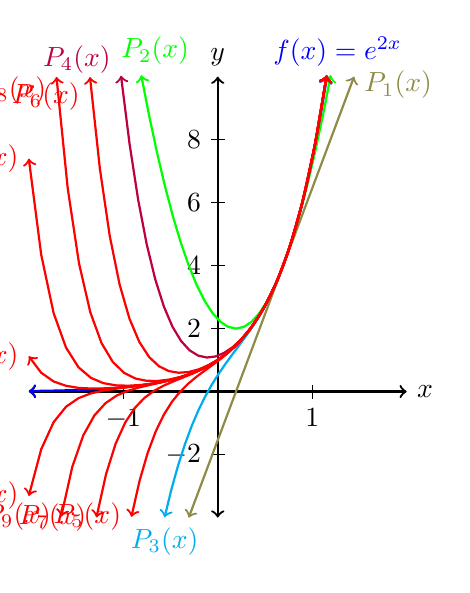
\begin{tikzpicture}
    [
        x=1.2cm,y=0.4cm,
        declare function={f(\x)=exp(2*\x);},
    ]
    \tikzmath{
        \lntwo = ln(2);
        \c{0} = 4;
        int \i;
        for \i in {0,...,11}{
            int \j;
            \j = \i + 1;
            \c{\j} = \c{\i} * 2 / \j;
        };
        function T1(\x) { return \c{0} + \c{1} * (\x - \lntwo); };
        function T2(\x) { return T1(\x) + \c{2} * (\x - \lntwo)^2; };
        function T3(\x) { return T2(\x) + \c{3} * (\x - \lntwo)^3; };
        function T4(\x) { return T3(\x) + \c{4} * (\x - \lntwo)^4; };
        function T5(\x) { return T4(\x) + \c{5} * (\x - \lntwo)^5; };
        function T6(\x) { return T5(\x) + \c{6} * (\x - \lntwo)^6; };
        function T7(\x) { return T6(\x) + \c{7} * (\x - \lntwo)^7; };
        function T8(\x) { return T7(\x) + \c{8} * (\x - \lntwo)^8; };
        function T9(\x) { return T8(\x) + \c{9} * (\x - \lntwo)^9; };
        function T10(\x) { return T9(\x) + \c{10} * (\x - \lntwo)^5 * (\x - \lntwo)^5; };
        function T11(\x) { return T10(\x) + \c{11} * (\x - \lntwo)^6 * (\x - \lntwo)^5; };
        function T12(\x) { return T11(\x) + \c{12} * (\x - \lntwo)^6 * (\x - \lntwo)^6; };
    }
    % The axes
    \draw[<->,thick] (-2,0) -- (2,0) node[right]{$x$};
    \draw[<->,thick] (0,-4) -- (0,10) node[above]{$y$};
    \foreach \x in {-1,1}
    \draw[thin] (\x,2.5pt) -- (\x,-2.5pt) node[below]{$\x$};
    \foreach \y in {-2,2,4,6,8}
    \draw[thin] (2.5pt,\y) -- (-2.5pt,\y) node[left]{$\y$};
    % The function
    \draw[thick,<->,blue]
    plot[domain=-2:1.15129,smooth](\x,{f(\x)})
    node[above,xshift=4pt]{$f(x) = e^{2x}$};
    % Taylor polynomials
    \draw[thick,<->,yellow!50!black]
    plot[domain=-0.3069:1.44314](\x,{T1(\x)})
    node[overlay,right,yshift=-3pt]{$P_1(x)$};

    \draw[thick,<->,green]
    plot[domain=1.196:-0.81](\x,{T2(\x)})
    node[overlay,above,xshift=5pt]{$P_2(x)$};

    \draw[thick,<->,cyan]
    plot[domain=1.16:-0.563](\x,{T3(\x)})
    node[below]{$P_3(x)$};

    \draw[overlay,thick,<->,purple]
    plot[domain=1.155:-1.024](\x,{T4(\x)})
    node[above left,yshift=-3pt]{$P_4(x)$};

    \draw[overlay,thick,<->,red]
    plot[domain=1.153:-0.914](\x,{T5(\x)})
    node[left]{$P_5(x)$};

    \draw[overlay,thick,<->,red]
    plot[domain=1.153:-1.3525](\x,{T6(\x)})
    node[left,yshift=-7pt]{$P_6(x)$};

    \draw[overlay,thick,<->,red]
    plot[domain=1.153:-1.284](\x,{T7(\x)})
    node[left]{$P_7(x)$};

    \draw[overlay,thick,<->,red]
    plot[domain=1.153:-1.7068](\x,{T8(\x)})
    node[left,yshift=-5pt]{$P_8(x)$};

    \draw[overlay,thick,<->,red]
    plot[domain=1.153:-1.6572](\x,{T9(\x)})
    node[left]{$P_9(x)$};

    \draw[overlay,thick,<->,red]
    plot[domain=1.153:-2](\x,{T10(\x)})
    node[left]{$P_{10}(x)$};

    \draw[overlay,thick,<->,red]
    plot[domain=1.153:-2](\x,{T11(\x)})
    node[left]{$P_{11}(x)$};

    \draw[overlay,thick,<->,red]
    plot[domain=1.153:-2](\x,{T12(\x)})
    node[left]{$P_{12}(x)$};
\end{tikzpicture}

\end{document}
